\documentclass{sig-alternate-2013}

\setlength{\paperheight}{11in}
\setlength{\paperwidth}{8.5in}

\usepackage[utf8]{inputenc}

\usepackage{amsmath,amssymb}
\usepackage{amsthmnoproof}
\usepackage{amsrefs}
\usepackage[usenames,dvipsnames]{color}
\usepackage{stmaryrd}
\usepackage{enumerate}
\usepackage[algoruled,vlined,english,linesnumbered]{algorithm2e}
\usepackage[pdfpagelabels,colorlinks=true,citecolor=blue]{hyperref}
\usepackage{comment}
\usepackage{multirow}
\usepackage{tikz}

\newcommand{\noopsort}[1]{}
\DeclareMathOperator{\NP}{NP}
\DeclareMathOperator{\HP}{HP}
\DeclareMathOperator{\PP}{PP}
\DeclareMathOperator{\Hom}{Hom}
\DeclareMathOperator{\End}{End}
\DeclareMathOperator{\GL}{GL}
\DeclareMathOperator{\val}{val}
\DeclareMathOperator{\pr}{pr}
\DeclareMathOperator{\tr}{Tr}
\DeclareMathOperator{\com}{Com}
\DeclareMathOperator{\Grass}{Grass}
\DeclareMathOperator{\Lat}{Lat}
\DeclareMathOperator{\round}{round}
\DeclareMathOperator{\rank}{rank}

\newcommand{\slp}{\text{\rm slp}}
\newcommand{\RS}{\text{\rm RS}}

\newcommand{\N}{\mathbb N}
\newcommand{\Z}{\mathbb Z}
\newcommand{\Zp}{\Z_p}
\newcommand{\Q}{\mathbb Q}
\newcommand{\Qp}{\Q_p}
\newcommand{\Fp}{\mathbb{F}_p}
\newcommand{\R}{\mathbb R}
\renewcommand{\O}{\mathcal O}
\newcommand{\OK}{\mathcal{O}_K}
\newcommand{\XX}{\mathbf X}
\newcommand{\trans}{{}^{\text t}}
\newcommand{\T}{\mathcal{T}}

\renewcommand{\prec}{\text{\rm prec}}

\newcommand{\id}{\textrm{id}}
\newcommand{\Epi}{\textrm{Epi}}
\renewcommand{\c}{\text{\rm c}}

\newcommand{\detp}{\det{'}}
\newcommand{\low}{\text{\rm low}}
\newcommand{\up}{\text{\rm up}}
\newcommand{\DI}{\text{\rm DI}}
\newcommand{\II}{\text{\rm II}}
\DeclareMathOperator{\charpoly}{char}
\newcommand{\charp}{\charpoly'}

\newcommand{\lb}{\ensuremath{\llbracket}}
\newcommand{\rb}{\ensuremath{\rrbracket}}
\newcommand{\lp}{(\!(}
\newcommand{\rp}{)\!)}
\newcommand{\col}{\: : \:}

\def\todo#1{\ \!\!{\color{red} #1}}
\definecolor{purple}{rgb}{0.6,0,0.6}
\def\todofor#1#2{\ \!\!{\color{purple} {\bf #1}: #2}}

\def\binom#1#2{\Big(\begin{array}{cc} #1 \\ #2 \end{array}\Big)}


\permission{%
}



\begin{document}

\newtheorem{theo}{Theorem}[section]
\newtheorem{lem}[theo]{Lemma}
\newtheorem{prop}[theo]{Proposition}
\newtheorem{cor}[theo]{Corollary}
\newtheorem{quest}[theo]{Question}
\newtheorem{conj}[theo]{Conjecture}
\theoremstyle{definition}
\newtheorem{rem}[theo]{Remark}
\newtheorem{ex}[theo]{Example}
\newtheorem{deftn}[theo]{Definition}

\title{Multiplication, division and factorization\\of p-adic polynomials}

\numberofauthors{3}
\author{
\alignauthor Xavier Caruso\\
  \affaddr{Universit\'e Rennes 1}\\
  \affaddr{\textsf{xavier.caruso@normalesup.org}}
\alignauthor David Roe \\
  \affaddr{University of Pittsburgh}\\
  \affaddr{\textsf{roed.math@gmail.com}}
\alignauthor Tristan Vaccon\\
  \affaddr{Rikkyo University}\\
  \affaddr{\textsf{vaccon@rikkyo.ac.jp}}
}

\maketitle

\begin{abstract}
\end{abstract}

\category{I.1.2}{Computing Methodologies}{Symbolic and Algebraic Manipulation -- \emph{Algebraic Algorithms}}
\terms{Algorithms, Theory}
\keywords{}

%\vspace{1mm}
% \noindent
% {\bf Categories and Subject Descripto\RS:} \\
%\noindent I.1.2 [{\bf Computing Methodologies}]:{~} Symbolic and Algebraic
%  Manipulation -- \emph{Algebraic Algorithms}
%
% \vspace{1mm}
% \noindent
% {\bf General Terms:} Algorithms, Theory
%
% \vspace{1mm}
% \noindent
% {\bf Keywords:} $p$-adic precision, linear algebra, ultrametric analysis
%\medskip

\section{Introduction}

\section{Modular multiplication}

\section{Euclidean division}

\begin{theo} \label{theo:EDivisionNP}
Here should be the theorem for the Newton polygons during a Euclidean division.
\end{theo}

\section{Slope factorization}
\subsection{Main theorem}

\begin{theo} \label{theo:slope-factor}
Under some assumptions... $\textrm{coeff}(P,d)=1,$ $\NP (A_0)' <0$ (???)

\begin{align*}
A_0 &= \textrm{trunc}(P,d), \\
B_{0} &= P \div A_{0}, \\
V_{0} &= 1.
\end{align*}


\begin{align*}
A_{i+1} &= A_i + (V_i P \% A_i), \\
B_{i+1} &= P \div A_{i+1}, \\
V_{i+1} &= (2 V_i -V_i^2 B_{i+1} ) \% A_{i+1}.
\end{align*}
$A_i$ convergences to $A_\infty$ such that $\NP (A_\infty)= \NP (A_0)$ and $A_\infty$ divides $P.$
\end{theo}

\begin{rem}
Using $P \mapsto P^*=X^{deg(P)}P \left( \frac{1}{X} \right), $ the assumptions in \ref{theo:slope-factor} do not induce any loss in generality.
\end{rem}

\subsection{Useful formulae}

\begin{lem}
Some definitions :
\begin{align}
R_i &= A_{i+1} -A_i, \label{eqdef:Ri}\\
S_i &= P \% A_i, \label{eqdef:Si} \\
Q_i &= V_i P \div A_i. \label{eqdef:Qi}. 
\end{align}
Some formulae :
\begin{align}
B_i-B_{i+1} &= R_i B_{i+1} \div A_i, \label{eqdef:Biminus} \\
S_i-S_{i+1} &= R_i B_{i+1} \div A_i,  \label{eqdef:Siminus} \\
S_{i} &= (B_i R_i + (1-V_i B_i) S_{i-1}+(1-V_i B_i)(S_i-S_{i-1})) \% A_{i}, \label{eqdef:Si2}  \\
V_{i+1}-V_i &= (V_i (1-V_i B_i)+V_i^2(B_i-B_{i+1})) \% A_{i}, \label{eqdef:Viminus}\\
1-Q_i &= (1-V_i B_i)+((R_i-V_i S_i) \div A_i), \label{eqdef:Qiminus}\\
R_{i+1} &= ((V_{i+1}-V_i)S_{i+1}+(1-Q_i)R_i) \% A_{i+1}, \label{eq:Riplus}\\
1-V_{i+1}B_{i+1} &= ((1-V_i B_i)+V_i (B_i-B_{i+1}))^2. \label{eq:ViBiplus}
\end{align}
\end{lem}
\begin{proof}
We first remark that by definition,
\begin{align*}
P &= A_i B_i + S_i, \\
P V_i&= A_i Q_i + R_i.
\end{align*}
Since $P= A_i B_i + S_i= A_{i+1} B_{i+1} + S_{i+1},$ we have \[R_i B_{i+1}= (B_i -B_{i+1})A_i + (S_i+S_{i+1}).\]
Hence, by consideration of degree, what we have written is the Euclidean division of $R_i B_{i+1}$ by $A_i$ and we obtain \eqref{eqdef:Biminus} and \eqref{eqdef:Siminus}.

From $V_i P =  A_i Q_i + R_i=V_i (A_i B_i + S_i),$ we get \begin{equation}(V_i B_i -Q_i) A_i=R_i-V_i S_i. \label{eq:ViBiQi} \end{equation} Thus, \[ R_i=V_i S_i \% A_i.\]
Hence, $B_i R_i =S_i (V_iB_i-1)+S_i \% A_i,$ and $S_i=B_i R_i-S_i (V_iB_i-1) \% A_i.$ \eqref{eqdef:Si2} follows directly.

By definition of $V_i,$ we get $V_{i+1}-V_i=V_i (1-V_i B_{i+1}) \% A_{i+1}.$ \eqref{eqdef:Viminus} follows immediately.

We can write $1-Q_i=(1-V_i B_i)+(V_i B_i - Q_i).$ Using \eqref{eq:ViBiQi}, we get \eqref{eqdef:Qiminus}.

We have $V_i P=A_i Q_i+R_i=(A_{i+1}-R_i)Q_i+R_i,$ and $V_{i+1} P=A_{i+1} Q_{i+1}+R_{i+1}.$ As a consequence, 
\begin{align*}
R_{i+1} &= (V_{i+1}-V_i)P+(1-Q_i)R_i \\
 &= (V_{i+1}-V_i)S_{i+1}+(1-Q_i)R_i) \% A_{i+1},
\end{align*} and \eqref{eq:Riplus} is proved.

Finally, \begin{align*}
1-V_{i+1}B_{i+1} &= 1-2V_i B_{i+1}+V_i^2 B_{i+1}^2 \% A_{i+1}, \\
&= (1-V_i B_{i+1})^2 \% A_{i+1}, \\
&= ((1-V_i B_i)+V_i (B_i-B_{i+1}))^2 \% A_{i+1},
\end{align*} which concludes the proof.
\end{proof}

\begin{deftn}
Notation:
\[P=-d \lambda_0+d \slp(\lambda_0) + l_1 \slp (\lambda_1)+\RS \]
($\RS$ for remaining slopes)

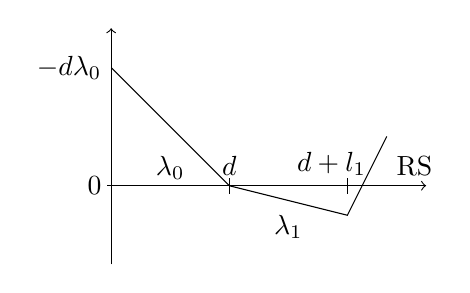
\begin{tikzpicture}
\draw[->] (0,-1) -- (0,2);


\draw[->] (-0.05,0) -- (4,0);

\node[left] at (0,0) {$0$};

\draw (1.5,-.1) -- (1.5,.1);
\node[above] at (1.5,0) {$d$};

\draw (3,-.1) -- (3,.1);
\node[above] at (2.8,0) {$d+l_1$};

\node[left] at (0,1.5) {$-d \lambda_0$};

\draw (0,1.5)-- (1.5,0) -- (3,-.375)-- (3.5,.625);
\node[below] at (.75,0.5) {$\lambda_0$};
\node[below] at (2.25,-0.25) {$\lambda_1$};
\node[right] at (3.5,0.25) {$\RS$};
\end{tikzpicture}
\end{deftn}

\subsection{Proof of the Main Theorem}

\subsubsection{Initial Newton polygons}

\begin{lem}
$\NP(R_0)=\NP(S_0)$:
\[ \NP (R_0)=\NP(S_0)=(\lambda_1-\lambda_0)- d \lambda_0+(d-1)\slp( \lambda_0). \]

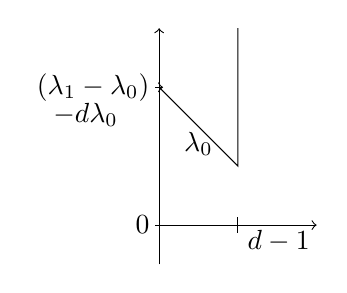
\begin{tikzpicture}
\draw[->] (0,-.5) -- (0,2.5);


\draw[->] (-0.05,0) -- (2,0);

\draw[->] (-0.05,1.75) -- (.05,1.75);
\node[left] at (0,1.75) {$(\lambda_1-\lambda_0)$};
\node[left] at (-.4,1.4) {$-d \lambda_0$};



\node[left] at (0,0) {$0$};


\draw (1,-.1) -- (1,.1);
\node[below, right] at (1,-.2) {$d-1$};


\draw (0,1.75) -- (1,.75) -- (1,2.5);
\node[below] at (.5,1.3) {$\lambda_0$};
\end{tikzpicture}

$\NP (1-V_0B_0 \% A_0)$:
\begin{align*}
\NP ((1-V_0B_0)\% A_0) &\geq (\lambda_1-\lambda_0)+1\slp( \lambda_0)+(d-1) \slp(\lambda_1), \\
&\geq (\lambda_1-\lambda_0)+d\slp( \lambda_0). \\
\end{align*} 
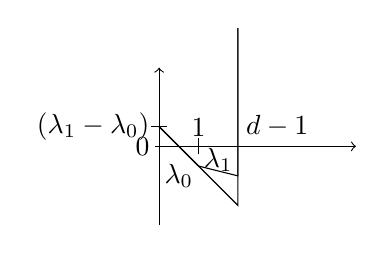
\begin{tikzpicture}
\draw[->] (0,-1) -- (0,1);


\draw[->] (-0.05,0) -- (2.5,0);

\node[left] at (0,0) {$0$};


\node[above] at (1.5,0) {$d-1$};

\draw (.5,-.1) -- (.5,.1);
\node[above] at (.5,0) {$1$};

\draw (-.1,.25) -- (.1,.25);
\node[left] at (0,.25) {$(\lambda_1-\lambda_0)$};

\draw (0,.25) -- (.5,-.25) -- (1,-.375)-- (1,1.5);
\draw (0,.25) -- (.5,-.25) -- (1,-.75)-- (1,1.5);



\node[below] at (.25,-0.1) {$\lambda_0$};
\node[below] at (.75,0.1) {$\lambda_1$};
\end{tikzpicture}



\end{lem}


\subsubsection{Unchanged Newton polygons}




\begin{lem}
$\NP (V_i)$ for $i>0$ ($V_0=1$):
\[\NP(V_i)=0+(d-1)\slp( \lambda_1). \]

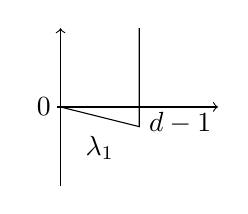
\begin{tikzpicture}
\draw[->] (0,-1) -- (0,1);


\draw[->] (-0.05,0) -- (2,0);

\node[left] at (0,0) {$0$};

\node[below, right] at (1,-.2) {$d-1$};


\draw (0,0) -- (1,-.25) -- (1,1);
\node[below] at (.5,-0.25) {$\lambda_1$};
\end{tikzpicture}

$\NP (B_i)$:
\[\NP(B_i)=0+(l_1)\slp( \lambda_1)+\RS. \]

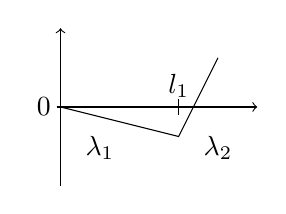
\begin{tikzpicture}
\draw[->] (0,-1) -- (0,1);


\draw[->] (-0.05,0) -- (2.5,0);

\node[left] at (0,0) {$0$};

\draw (1.5,-.1) -- (1.5,.1);
\node[above] at (1.5,0) {$l_1$};


\draw (0,0) -- (1.5,-.375) -- (2,.625);
\node[below] at (.5,-0.25) {$\lambda_1$};
\node[below] at (2,-0.25) {$\lambda_2$};
\end{tikzpicture}
\end{lem}

\subsubsection{Newton polygons inside the loop}

\begin{lem}
\begin{align*}
\NP (R_i), \NP(S_i) & \geq -\lambda_0+2^i(\lambda_1-\lambda_0)+(d-1) \slp (\lambda_0), \\
\NP (1-V_i B_i) & \geq 2^i (\lambda_1-\lambda_0)+(d-1) \slp (\lambda_0),\\
\NP (B_i-B_{i+1}) & \geq 2^i (\lambda_1-\lambda_0)+(\lambda_1-\lambda_0)+(l_1-1) \slp (\lambda_1)+\RS, \\
\NP (S_i-S_{i+1}) & \geq -\lambda_0 d+2^i (\lambda_1-\lambda_0)+(d-1) \slp (\lambda_0),\\
\NP (V_i-V_{i+1}) & \geq 2^i (\lambda_1-\lambda_0)+(d-1) \slp (\lambda_0),\\
\NP (1-Q_i) & \geq  2^i (\lambda_1-\lambda_0)+(d-1) \slp (\lambda_0).\\
\end{align*}
\end{lem}


\end{document}
